\chapter{Setting up networking}
\label{chp:setting-up-networking}
\ProductName{} can run with jobs and variables shared between 2 or more Unix
hosts, possibly different platforms. To do this, networking needs to be enabled.

Networking also needs to be enabled if you intend to use:

\begin{itemize}
\item The API, whether for Unix or MS Windows
\item The MS Windows clients \IfXi{whether the PyQt version or the Visual C++ version}
\end{itemize}

To use any or all of these things, \ProductName{} must be run in network mode.

It does \textbf{not} need to be enabled if you have a standalone computer and only run the standard clients, i.e.
the shell, curses, GTK+ or Motif interfaces.

\IfXi{Whether networking is enabled or not is determined by the licence key. You can quickly check if it is enabled by
running \PrXbChecklic. The output will normally be as follows:

\begin{expara}
This copy is for: Acme Systsems

Serial is 123456

Start time 13:00:00 27/04/2013

No limit

Validated for networks

\end{expara}

The last line will not be displayed if the licence is not networked.

If the copy is network-enabled and should not be or vice versa, you should obtain a new key and re-license the product
using \PrXbVwrite.}
\IfGNU{When \ProductName{} is normally installed, all the networking facilities are included. However it may be started, if required,
without networking by providing the \exampletext{\-n} option to \progname{btsched}. However \PrBtstart{} does not currently support
this, so \progname{btsched} may have to be started ``by hand''.}

\warnings{If \ProductName{} was previously started non-networked and is restarted with networking enabled, all the jobs and
variables intended to be exported will have to be reset, as the exported flag will be turned off by being started non-networked.}

In order for the networking facility to work correctly, three things have to be done:

\begin{enumerate}
\item Some standard ``service'' names need to be inserted in the \filename{/etc/services} file.
\item Hosts may need to be configured in a hosts file \hostsfile{}.
\item The product needs to be \IfXi{given a ``network licence''}\IfGNU{started in network mode}.
\end{enumerate}
When you install \ProductName{} \IfXi{with a network licence using the standard install script}\IfGNU{normally}, these items are all
attended to.

\IfXi{If you have already installed a non-network licence, and want to change, you may find it easiest to just re-install
by running the installation script, but answering the question differently.

The services will be set up appropriately, and a network licence installed.}

\section{Editing the host file}
Unlike earlier versions of \ProductName{}, you probably only need to edit the
host file if:

\begin{enumerate}
\item You need to set up a ``local address'', the IP address by which the host you are
installing on is known to the outside world. This is needed as jobs and variables are identified partly by that IP address.
\item You want to give convenient aliases to other hosts you inter-connect with.
\item You want to denote some fixed IP addresses as clients only, not expecting to receive information about jobs
and variables (typically for Windows clients). 
\end{enumerate}
An additional use, of declaring mappings from Windows user names to UNIX user names, is still supported, but
deprecated in favour of the use of the user map file, \usermap{} for this purpose.

A special host editor program \PrHostedit{} (plus a GUI version of it \PrXhostedit) is available to
edit the host file. This currently still understands and maintains deprecated facilities.
\IfXi{These are now put with the other user-level binaries.}

Note that the discussion below is for \PrHostedit{} rather than \PrXhostedit{} as the latter may not always be available
if GTK+ is not available on your system. If you have \PrXhostedit{} available, you may want to try using that, hopefully the
menu selections will be obvious from the discussion below.

To run this enter:

\begin{expara}

\HosteditName{} -I \hostsfilename

\end{expara}

The \exampletext{-I} denotes that the file should be edited in place.

With a new installation, the display will take the following form:

\begin{figure}
\centering
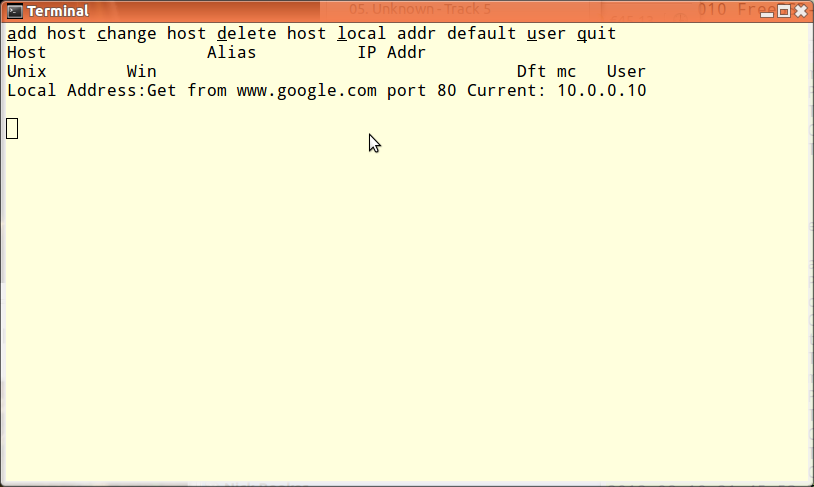
\includegraphics[width=16.999cm,height=10.169cm]{img/he1.png}
\end{figure}
The installation script sets up the hosts file to obtain the local IP
address by connecting to \filename{www.google.com}.

\subsection{Setting up the local address}
An important aspect of the network code is to obtain the local address.

Jobs and variables owned by the server are distinguished from similar jobs and variables on other
servers by the IP address. The server needs to know what its own address is from the point of view
of other servers, in order that it can deal with references to its own jobs and variables.

We call this IP address the ``local address''. It is sometimes not obvious, especially if the
server can be referred to by different IP addresses.

Without a hosts file present, \ProductName{} will try to discover the local
address by applying \exampletext{gethostbyname} to the result
of \exampletext{gethostname}. However this often yields a ``loopback'' IP address such as
\filename{127.0.0.1} rather than something identified to other hosts.

To overcome this, you can set up in the host file:

\begin{enumerate}
\item An explicit IP address or host name yielding an IP address to use or
\item A host name or IP address to connect to (usually using the HTTP port) and get the local IP address from
\exampletext{getsockname}.
\end{enumerate}
The latter (more recently introduced) is better, especially on hosts which may have a variable DHCP-assigned IP address
which may change between reboots.

To set up a fixed local address, type \userentry{l}.

If there is a local address you will be asked:

\begin{expara}

Local address set, do you want to unset it? [N]

\end{expara}

Type \userentry{y} to unset this prior to setting a new one by typing \userentry{l} again.

If there is no local address set, or you have just unset it, you should get the message

\begin{expara}

Do you want to set a local address? [N]

\end{expara}

Type \userentry{y} and you will get the prompt

\begin{expara}

Local address:

\end{expara}

Now you can type the host name or IP address to use.

\subsection{Setting up the local address from a website}
Rather than typing in a local address, you can obtain the local address by connecting to a website and noting the local address using
\exampletext{getsockname}.

You can do this once, or you can do it every time (this is best if the IP address may change, due to it being set by DHCP).

Type \userentry{w} to select this option, and receive the message:

\begin{expara}

Use Google? [N]

\end{expara}

If you reply \userentry{N} to this, you will be prompted for another host. If you reply \userentry{Y}, then
\filename{www.google.com} will be used.

In either event (after checking that the host is valid and has an HTTP server on port 80), you will get the prompt:

\begin{expara}

Always get host that way? [Y]

\end{expara}

If you reply \userentry{Y} to this, it will set up to always obtain the local address from that host when \ProductName{} starts, otherwise
it will just set the local address IP as if it had been explicitly entered.

\subsection{Setting up the local address from a connected host}
If you have already set up a local host, you can use one of those to set
the local address and possibly always do so by moving the cursor to it
and typing \userentry{L}.

A variety of possible ports and services are tried and the first one to
which a connection can be made is used.

Again you will be asked if you always want to get the host that way.

\subsection{Adding a host}
You should add a host:

\begin{enumerate}
\item If you want to give a name to an IP address by which the host is referred to.
\item If you want to give a more convenient name to a host rather than a fully-qualified domain name.
\item If you want to arrange for the host to be automatically connected on startup.
\item If you want to say that a given host is only to be used for clients.
\end{enumerate}
We don't recommend that you set up Windows client user names any more, instead use the User Map file \usermap.

Press ``\userentry{a}'' to add a host, you should get the prompt:

\begin{expara}

Is new entry a Unix host(Y) or Client(N)? [Y]

\end{expara}

Just press ENTER. Next you should get the prompt.

\begin{expara}

Unix host name:

\end{expara}

Type the name of the host, e.g. on our site, one is called \filename{jessie}. You should then
get the prompt:

\begin{expara}

Any alias for jessie:

\end{expara}

Unless you require an alias, just press ENTER. Next you will get the prompt:

\begin{expara}

Probe (check alive) before connecting? [Y]

\end{expara}

Again press ENTER (this checks that the host is on-line before
attempting a TCP connection, however in some cases a Firewall etc
prevents UDP messages from getting through and this must be avoided.

\begin{expara}

Trust host with user information? [Y]

\end{expara}

The function of this has now been deprecated, just accept it.

\begin{expara}

Manual Connections only? [N]

\end{expara}

This concerns whether you want the connection to the other Unix host to be attempted as soon as \ProductName{} is started, or manually by means of \PrBtconn. Reply \userentry{y} if you require this.

\begin{expara}

Default timeout value OK? [Y]

\end{expara}

Press ENTER unless you want a variation in the connection timeout. The display should now look like this:

\begin{figure}
\centering
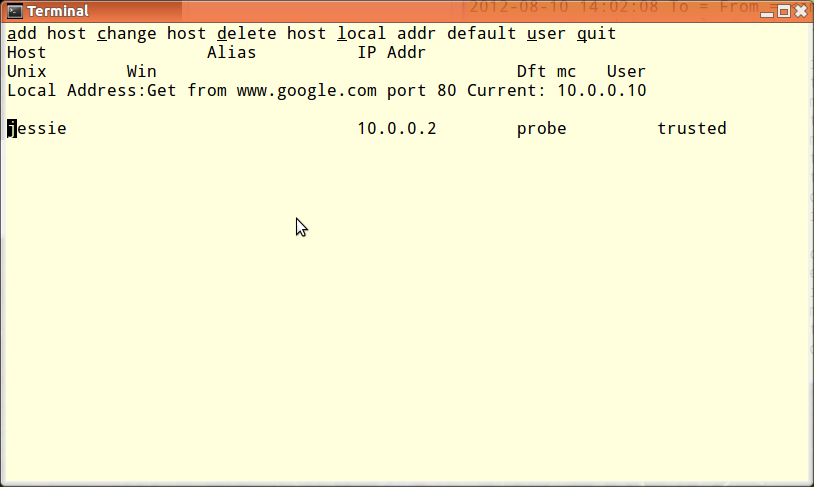
\includegraphics[width=16.999cm,height=10.169cm]{img/he2.png}
\end{figure}
This should be repeated for each host (and should also be repeated on each host so configured). To make any amendments, move the cursor to
the relevant host name and type \userentry{c} or to delete it type \userentry{d}.

\subsection{Adding a fixed IP address Windows host}
Press \filename{a} to add a host name, and this time type
\filename{n} to indicate that a Windows host is being added.
The prompts are as follows:

\begin{expara}

Specific Windows Host (Y) or {\textasciigrave}roaming
user{\textquotesingle} (N)? [Y]

\end{expara}

Press ENTER to denote a specific IP address.

\begin{expara}

Windows client host name:

\end{expara}

Type the name of the hosts, e.g. ``kim''.

\begin{expara}

Any alias for kim:

\end{expara}

Again, press ENTER unless you want to give an alias.

\begin{expara}

Default user:

\end{expara}

This is prompting for a default user name to be used for access --- the
normal UNIX user of that PC, although other users can use it,
specifying a password. This can be omitted if required.

\begin{expara}

Password-check user(s)? [N]

\end{expara}

This can be turned on to force password-checks on all users if required.

\begin{expara}

Default timeout value OK? [Y]

\end{expara}

Again, this can be left as the default or not (it is slightly more
important, as if the password checks are enabled, it gives the time
after which the user will have to log in again with his password if he
has not done anything in the meantime).

\subsection{Adding a DHCP client}
Please note that this has been deprecated in favour of using a user
mapping file, but is included for compatibility with previous versions.
If both are specified, the hosts file, which is read second, will take
priority.

This is where the IP may change each time and the recognition is by the
user name (or possibly a Windows user name matched to a Unix user
name).

Again, press \userentry{a} to add a host name and
\userentry{n} to indicate that a Windows host is being added,
and now type \userentry{n} again to select DHCP clients.

\begin{expara}

Unix user name:

\end{expara}

This is the user id under which activities will be run on the Unix host.
Be careful to make the case of characters correct (usually all lower
case).

\begin{expara}

Windows user name:

\end{expara}

This is the windows user name, or blank if the same as the Unix user
name. It is not case-sensitive.

\begin{expara}

Do you want to specify a default machine name? [N]

\end{expara}

This enables the user to specify the (Unix) host name of the usual PC at
which the user works. He or she will be able to ``log in'' at other hosts with the password.

\begin{expara}

Password-check user(s)? [N]

\end{expara}

You can set this to insist on a password in all cases.

\begin{expara}

Default timeout value OK? [Y]

\end{expara}

Again this gives the timeout value. After this time of inactivity, the
user will have to log in again.

\subsection{Quitting and saving}
Type \userentry{q} to quit and save the newly-created hosts file in \hostsfile{}.

\subsection{Editing the hosts file after installation}
The utility \PrHostedit{} (or \PrXhostedit)may be used to edit the hosts file.

We recommend that \ProductName{} be halted and restarted after this has been
completed.

To invoke it, use the following command:

\begin{expara}

\HosteditName{} -I \hostsfilename

\end{expara}

The \exampletext{{}-I }argument denotes that the file is to be edited in place.

\section{User map file}
The user map file provides a mapping between external names, usually Windows user names, and UNIX names.

The file is in \usermap, and consists (apart from comments introduced by the \filename{\#} character) of
lines of the format

\begin{expara}

unix-user:windows-user

\end{expara}

For example:

\begin{expara}

\# User mapping file

jmc:john collins

sec:sue collins

guest:default

\end{expara}

The final entry gives a default user if a named user is not found in the file.

UNIX users not found on the host are silently ignored.

Any number of Windows users may be mapped to the same Unix user.

